\documentclass[11pt]{article}

\usepackage{fullpage}
\usepackage{rotating}   
\usepackage{amsmath}
\usepackage{amssymb}
\usepackage{amsthm}
\usepackage{fancyhdr}
\usepackage{algorithm}
\usepackage{algorithmic}
\usepackage{bm}
\usepackage{listings}
\usepackage{graphicx}
\usepackage{caption2}
\usepackage{subfigure}
\usepackage{float}
\usepackage{extpfeil}
\usepackage{color}
\usepackage[usenames,dvipsnames]{xcolor}


\newtheorem{theorem}{Theorem}[section]
\newtheorem{lemma}[theorem]{Lemma}
\newtheorem{corollary}[theorem]{Corollary}
\newtheorem{proposition}[theorem]{Proposition}
\newtheorem{definition}[theorem]{Definition}
\newtheorem{conjecture}[theorem]{Conjecture}
\newtheorem{remark}[subsection]{Remark}

%%
\newcommand\numberthis{\addtocounter{equation}{1}\tag{\theequation}}

%% define new symbols
\def\bx{\bm{x}}
\def\bb{\bm{b}}
\def\ba{\bm{a}}
\def\bc{\bm{c}}
\def\bf{\bm{f}}
\def\by{\bm{y}}
\def\bu{\bm{u}}
\def\bv{\bm{v}}
\def\BW{\bm{W}}
\def\BA{\bm{A}}
\def\bz{\bm{z}}
\def\BZ{\bm{Z}}
\def\BH{\bm{H}}
\def\BL{\bm{L}}
\def\BU{\bm{U}}
\def\BV{\bm{V}}
\def\BB{\bm{B}}
\def\BC{\bm{C}}
\def\BD{\bm{D}}
\def\BE{\bm{E}}
\def\BW{\bm{W}}
\def\BQ{\bm{Q}}
\def\BG{\bm{G}}
\def\BA{\bm{A}}
\def\BX{\bm{X}}
\def\BY{\bm{Y}}
\def\BQ{\bm{Q}}
\def\BI{\bm{I}}
\def\BR{\bm{R}}

%% define new brackets
\def\la{\left\langle}
\def\ra{\right\rangle}
\def\ln{\left\|}
\def\rn{\right\|}
\def\lb{\left(}
\def\rb{\right)}
\def\lsb{\left[}
\def\rsb{\right]}
\def\lcb{\left\{}
\def\rcb{\right\}}

%%
\DeclareMathOperator*{\argmin}{arg\,min}
\DeclareMathOperator*{\argmax}{arg\,max}

%%
\title{Homework XI}
\author{Name: Shao Yanjun, Number: 19307110036}


\begin{document}
\maketitle

%------------------------------------
\begin{abstract}
This is Daniel's homework of  "Numerical Algorithms with Case Studies II".
\end{abstract}
%-------------------------------------
%=====================
\section{Problems}
\paragraph{Q1}
We just verify this assumption with $n$ eigenvectors $x_j=\begin{pmatrix}
	1 & \omega_n^j & \omega_n^{2j} & \cdots &\omega_n^{(n-1)j}
\end{pmatrix}^T$ where $j=0,1,2,\cdots,n-1$ and $\omega_n=e^{-i\frac{2\pi}{n}}$
\begin{align}
	\begin{pmatrix}
		0 & 1 &   &  &\\
		  & 0 & 1 &  &\\
	      &  &\ddots&\ddots\\
		  &  &   &0 &1\\
		1 &  &   &  &0
	\end{pmatrix}
	\begin{pmatrix}
		1 \\
		\omega_n^j\\
		\omega_n^{2j}\\
		\cdots\\
		\omega_n^{(n-1)j}
	\end{pmatrix}
	=\begin{pmatrix}
		1 \\
		\omega_n^j\\
		\omega_n^{2j}\\
		\cdots\\
		\omega_n^{(n-1)j}
	\end{pmatrix} w_n^j
\end{align}
And so we will see that,
\begin{align}
	F^{-1}_nJ_nF_n=diag\{1,\omega_n^1,\omega_n^{2},\cdots,\omega_n^{(n-1)}\}
\end{align}
\paragraph{Q2}
First of all, we will explain why two-sided power spectrum appear on the plot. Discrete Fourier transformation can be intepreted as follows.
\begin{align}
	X(f)=\sum_{k=0}^{N}x(k)e^{-i\frac{2\pi fk}{N}}=\sum_{k=N}^{0}x(N-k)e^{-i\frac{2\pi f(N-k)}{N}}=\sum_{k=0}^{N}x(k)e^{i\frac{2\pi fk}{N}}=X(-f)=X(N-f)
\end{align}
Eliminate the higher mirrored copy of peaks. And check it with Matlab plots, only one peak for $sin(3x)$, while $sin(x)+sin(\sqrt[12]{128}x)$ has two peaks.
\begin{figure}[H]
 	\centering
 	\subfigure[$sin(3x)$]{
 		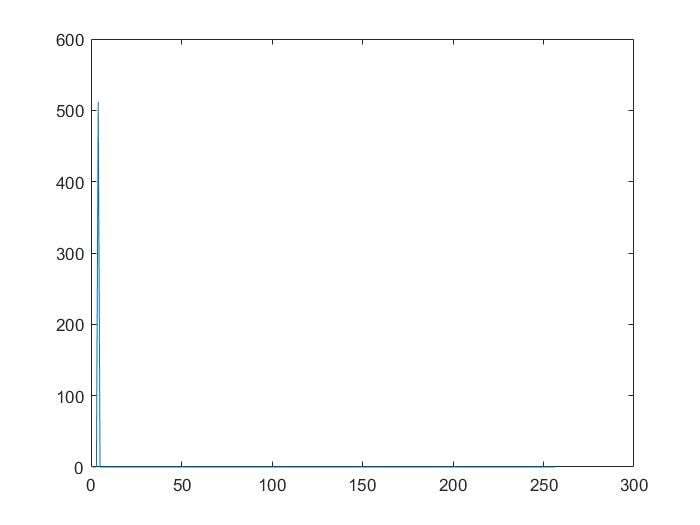
\includegraphics[width=0.4\linewidth]{p1.jpg}
 	}
 	\subfigure[$sin(x)+sin(^{12}\sqrt{128}x)$]{
 		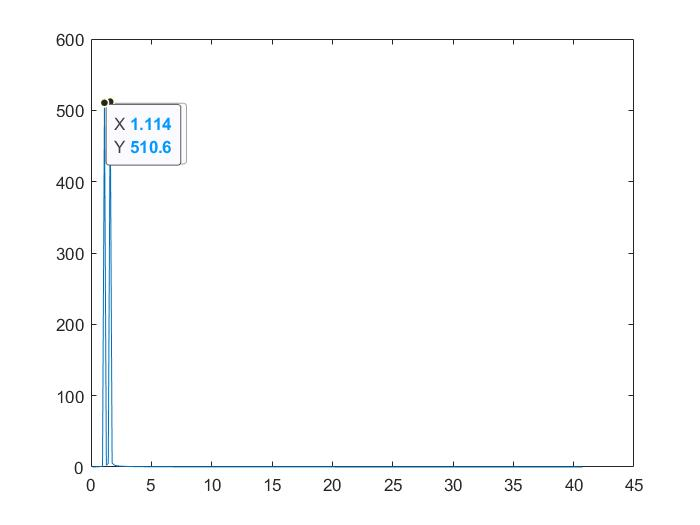
\includegraphics[width=0.4\linewidth]{p2.jpg}
 	}
\end{figure}
\paragraph{Q3}
The convolution theorem based on DFT is describe as follows,
\begin{align}
	\widehat{u*v}_k=\widehat{u}_k\cdot\widehat{v}_k
\end{align}
Represent $\widehat{u*v}_k$ using DFT formula,
\begin{align}
	(u*v)_k&=\sum_{j=0}^{N-1}u(j)\cdot v(k-j)\\
	&=\sum_{j=0}^{N-1}(\frac{1}{N}\sum_{n=0}^{N-1}U(n)\cdot e^{i\frac{2\pi nj}{N}})
	(\frac{1}{N}\sum_{m=0}^{N-1}V(m)\cdot e^{i\frac{2\pi m(k-j)}{N}})\\
	&=\frac{1}{N}\sum_{n=0}^{N-1}\sum_{m=0}^{N-1}U(n)V(m)\cdot e^{i\frac{2\pi mk}{N}}(\frac{1}{N}\sum_{j=0}^{N-1}e^{i\frac{2\pi (n-m)j}{N}})
\end{align}
And we also have the following Lemma that,
\begin{align}
	\sum_{j=0}^{N-1}e^{i\frac{2\pi (n-m)j}{N}}&=\sum_{j=0}^{N-1}(e^{i\frac{2\pi (n-m)}{N}})^j\\
	&=\frac{1-(e^{i\frac{2\pi (n-m)}{N}})^N}{1-e^{i\frac{2\pi (n-m)}{N}}}\\
	&=\begin{cases}
		0&\mbox{if $m\ne n$}\\
		1&\mbox{if $m=n$}
	\end{cases}
\end{align}
Therefore, we also have,
\begin{align}
	(u*v)_k&=\frac{1}{N}\sum_{n=0}^{N-1}\sum_{m=0}^{N-1}U(n)V(m)\cdot e^{i\frac{2\pi mk}{N}}(\frac{1}{N}\sum_{j=0}^{N-1}e^{i\frac{2\pi (n-m)j}{N}})\\
	&=\frac{1}{N}\sum_{n=0}^{N-1}U(n)V(n)\cdot e^{i\frac{2\pi nk}{N}}\\
	&=\widehat{\widehat{u}_k\cdot\widehat{v}_k}
\end{align}
Which means $\widehat{u*v}_k=\widehat{u}_k\cdot\widehat{v}_k$
\paragraph{Q4}
The correctness of myconv() is guaranteed by conv(). We use tic and toc in Matlab to examine the time consumption of conv() and myconv().
\begin{figure}[H]
	\centering
	\subfigure[Comparison]{
		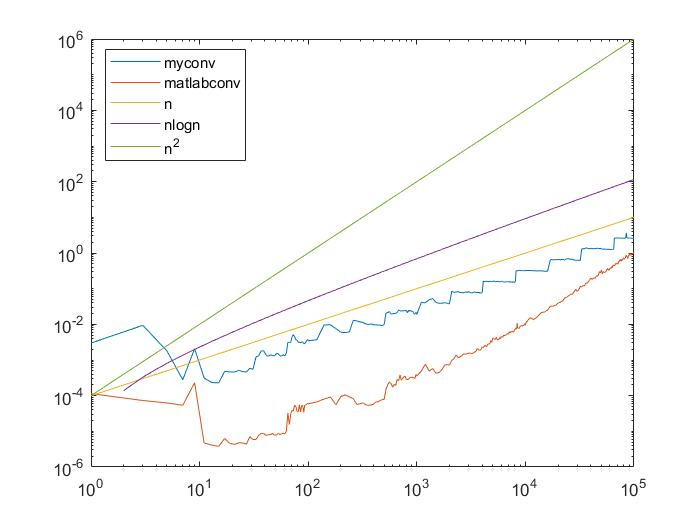
\includegraphics[width=0.8\linewidth]{s.jpg}
	}
\end{figure}
Surprisingly, the Matlab conv() is $O(n^2)$ level algorithm, while myconv() is indeed approximately $O(nlogn)$. It's natural to think that myconv() will definitely perform better than conv() for large problems.
\paragraph{Q5}
We construct wierd() to generate a insanely and randomly discontinuous function. Use $\sigma=\{1,10^{-1},10^{-2},10^{-3}\}$ from Gaussian function family $\phi(x)=\dfrac{1}{\sqrt{2\pi}\sigma}e^{-\dfrac{x^2}{2\sigma^2}}$
\begin{figure}[H]
	\centering
	\subfigure[Comparison1]{
		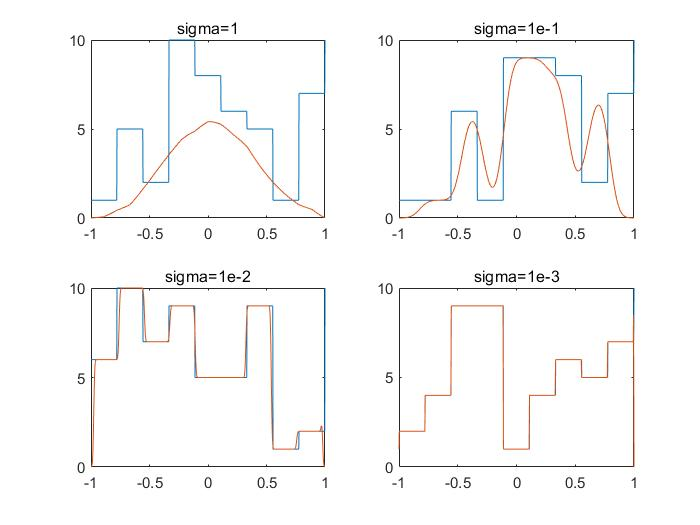
\includegraphics[width=0.4\linewidth]{good.jpg}
	}
	\subfigure[Comparison2]{
		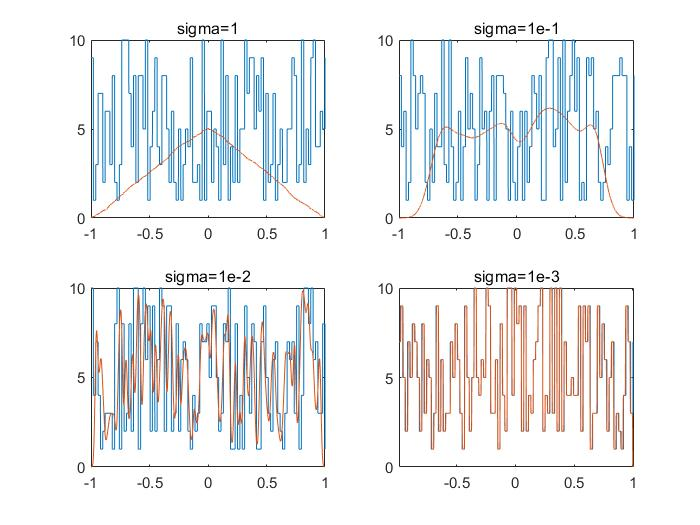
\includegraphics[width=0.4\linewidth]{good2.jpg}
	}
\end{figure}
\paragraph{Q6}
The audio file and every single tone is divided into small parts using some trivial techniques.
\begin{figure}[H]
	\centering
	\subfigure[signal]{
		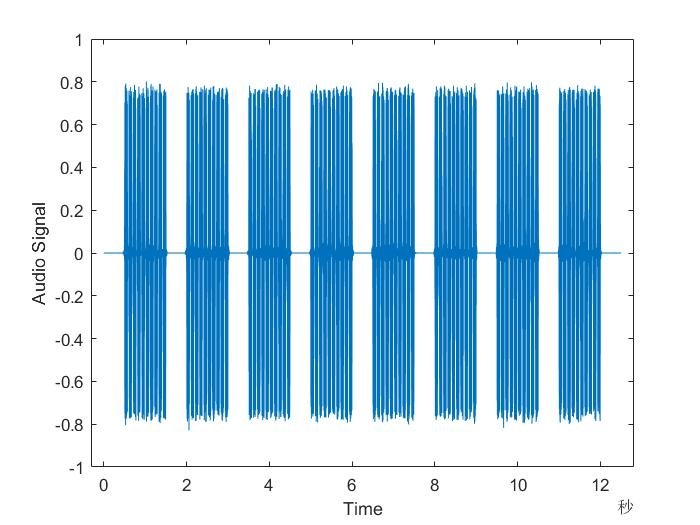
\includegraphics[width=0.4\linewidth]{mysignal.jpg}
	}
	\subfigure[division]{
		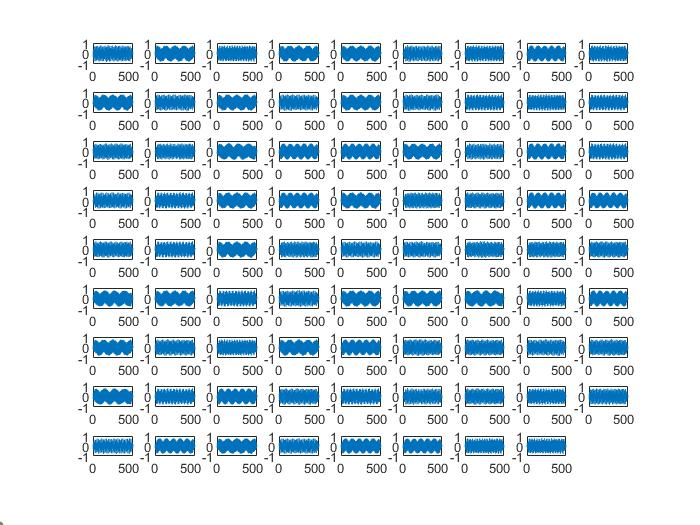
\includegraphics[width=0.4\linewidth]{division.jpg}
	}
\end{figure}
Using fft(). Note that the frequency corresponds to the signal frequency, which is $j\cdot fs$.
\begin{figure}[H]
	\centering
	\subfigure[signal FFT]{
		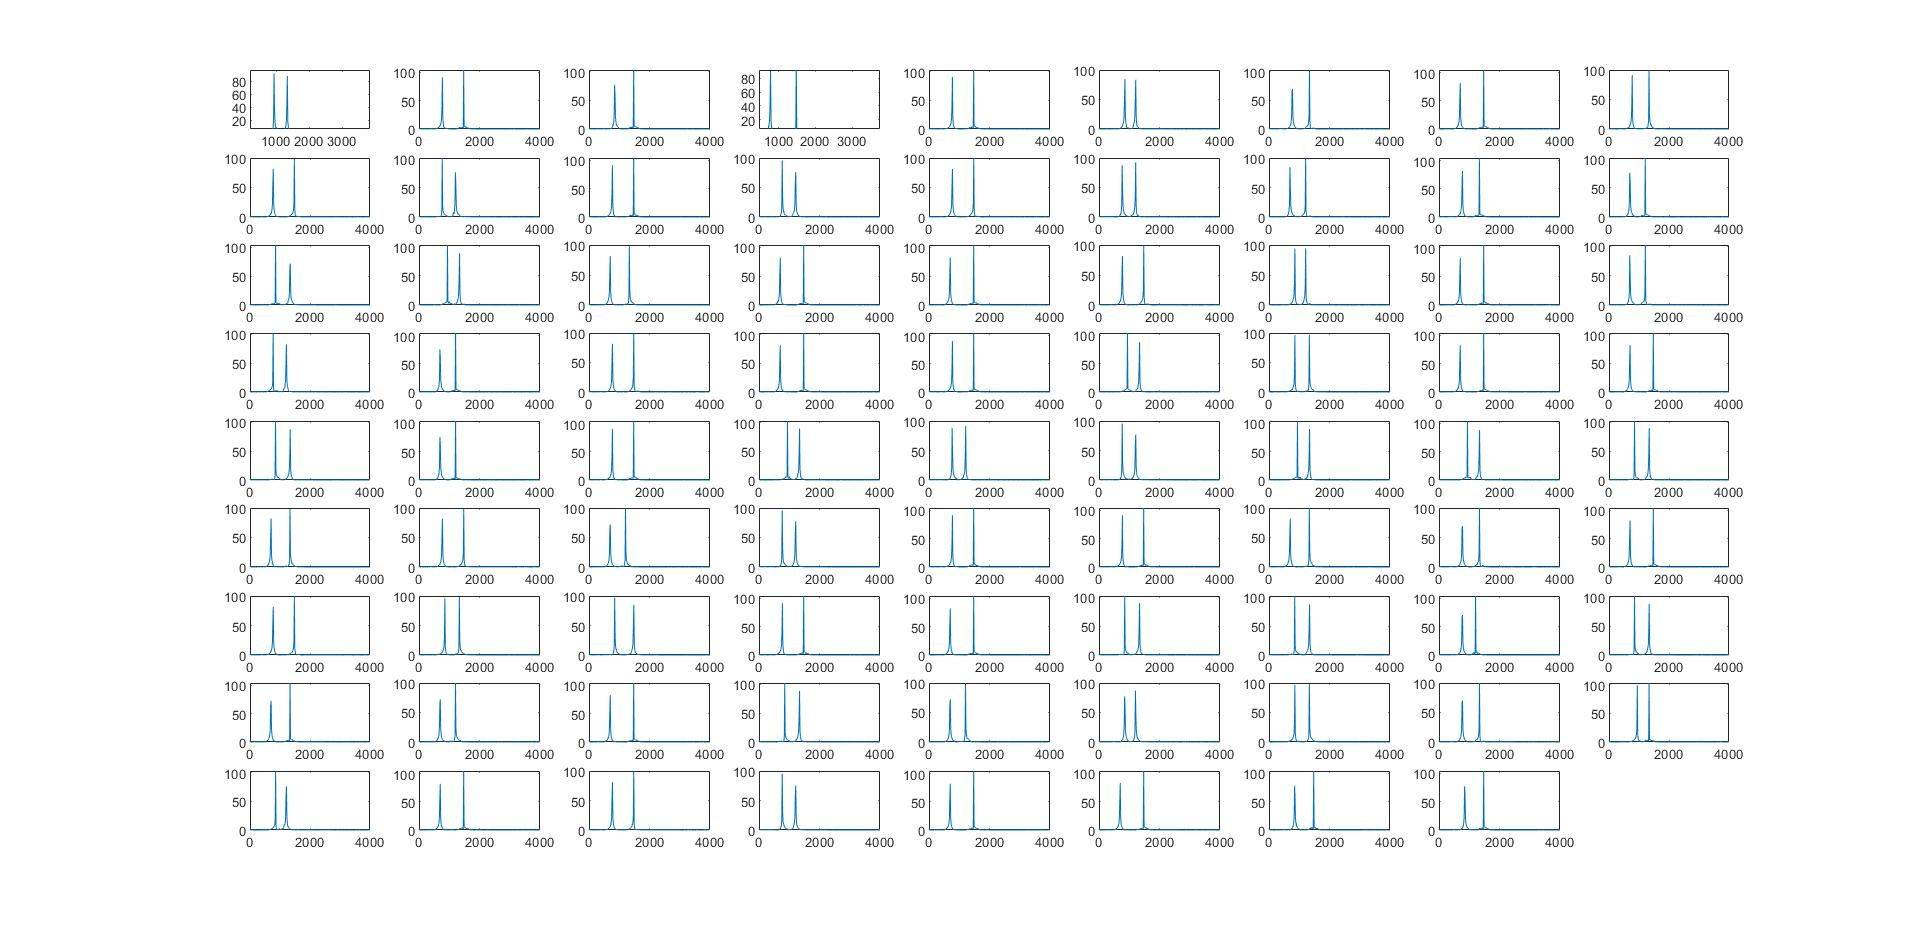
\includegraphics[width=0.8\linewidth]{signalfft.jpg}
	}
\end{figure}
The higher part of frequency can be ignored because they are simply mirror copies of spikes. Determine the two peaks for every sound, and look up for approximation in the table, we have,
\begin{figure}[H]
	\centering
	\subfigure[signals in frequency]{
		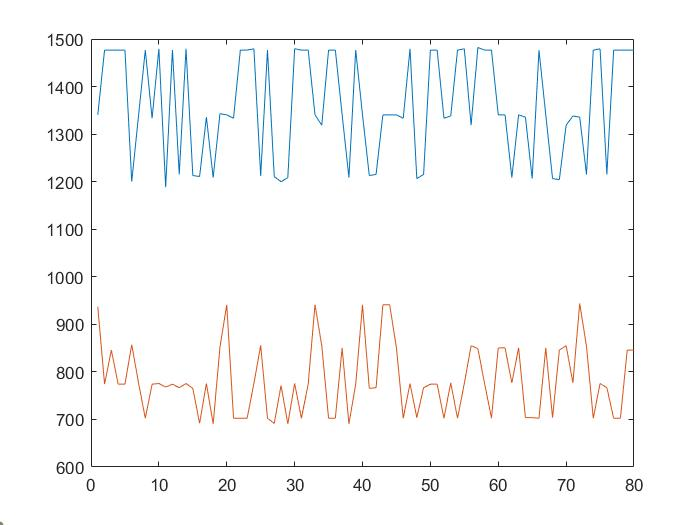
\includegraphics[width=0.8\linewidth]{mysignal_fre.jpg}
	}
\end{figure}
The recovered keys are "0696675356 4646415180 2336731416 3608338160 4400826146 6253689638 8482138178 5073643399".

\paragraph{Q8}
The comparison of myfft3() and myfft5() with fft() in Matlab.
\begin{figure}[H]
	\centering
	\subfigure[Comparison3]{
		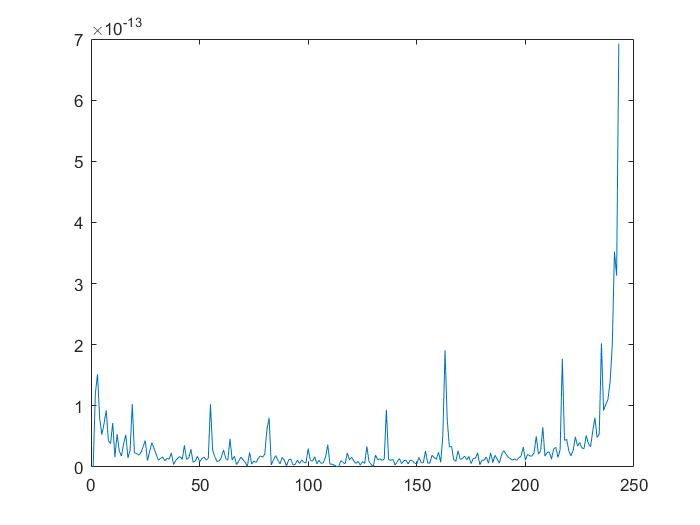
\includegraphics[width=0.4\linewidth]{error3.jpg}
	}
	\subfigure[Comparison5]{
		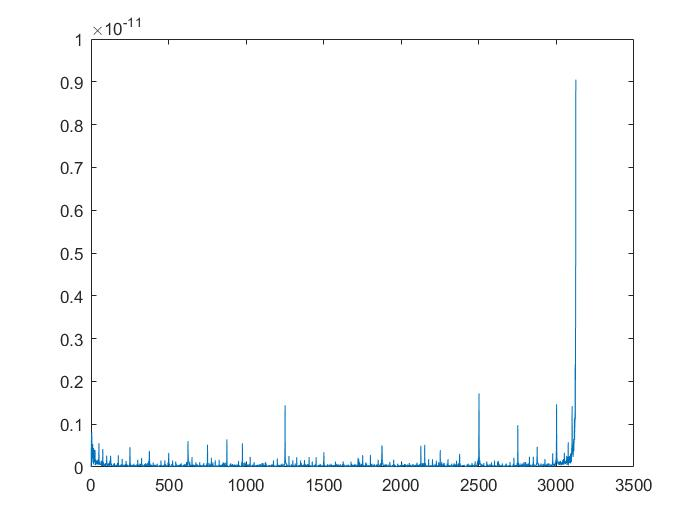
\includegraphics[width=0.4\linewidth]{error5.jpg}
	}
\end{figure}
%-------------------------------------
%=====================
\end{document}
